\subsection{Sequences comparison}
\label{sec:pang}

\paragraph{Presentation}

Sequence comparison is an essential task in genomics, for example to search whether an unknown sequence can be found in a reference database. For instance, the software BLAST has enabled such comparisons for several decades now. Due to the considerable increase in the volume of available sequences, many successors have attempted to improve the underlying algorithm and/or take advantage of the parallelization capabilities of hardware architectures. 

We propose here to implement a version of the BLAST algorithm with no gap for the comparison of amino acid sequences on a PIM-type architecture. This version will be called PANG (Protein Alignment with No Gap) and the equivalent command line for the original BLAST would be

\begin{minted}[bgcolor=bg]{bash}
blastp -query <query.fasta> -subject <db.fasta> -ungapped -out <output> 
   -comp_based_stats F -evalue <evalue> -seg yes 
\end{minted}


\paragraph{Limitations encountered}
None: the BPL code can be fully architecture-agnostic.


\paragraph{Benchmarks} 

In the following, we will compare a PIM/SDK version of the PANG algorithm with a version implemented using BPL. Note that some heuristics differ slightly, so we will also examine the results themselves in addition to the performance aspects. 

We perform a comparison between the well-known SwissProt protein database and a subset of proteins from Arabidopsis thaliana. These two databases contain 563,082 and 15,873 proteins respectively, corresponding to a total of 202,799,066 and 6,788,821 amino acids. 
For both implementations, we used several different parameter settings, with E-values of 1e-3, 1e-6 and 1e-18 respectively.
For the SDK/UPMEM and BPL/UPMEM versions, one rank was used, corresponding to 64 DPUs.

\paragraph{Results}

We present the results in \tablename~\ref{tab:pang-results} that compares SDK and BPL implementation for an UPMEM architecture. 

\begin{table}[htbp]
    \centering
    \caption{Execution times for Arabidopsis thaliana vs. Swissprot}
    \label{tab:pang-results}
    \begin{tabular}{lrr}
    \toprule
    & PIM/SDK & PIM/BPL \\
    \midrule
    evalue=1e-3 & 1892 & 1615  \\
    \midrule
    evalue=1e-6 & 1785 & 1564  \\
    \midrule
    evalue=1e-18 & 1781 & 1523  \\
    \bottomrule
    \end{tabular}
\end{table}

The BPL version exhibits slightly better performance than the version implemented directly with the UPMEM SDK, 
which may be due to the slightly different heuristics used in the two implementations. 
To better assess this aspect, the Venn diagrams in figure [\ref{fig:pang-venn}]  illustrate the overlap between the [refId, qryId] pairs produced 
by the two versions. Most of the results are common to both versions, with some results specific to each implementation, likely as a consequence of the different heuristics employed. It can also be observed that for increasingly smaller evalues, the share specific to the BPL version decreases, so that the results obtained by the BPL version are almost included in the results obtained by the SDK version.
The fact that the SDK version produces more results may partly explain its slightly longer execution time.

\begin{figure}
    \centering
    \begin{minipage}{0.32\textwidth}
        \centering
        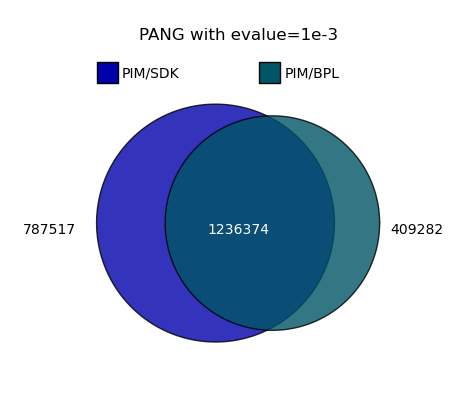
\includegraphics[width=1.1\textwidth]{fig_misc/pang.resulte3.png} % first figure itself
    \end{minipage}\hfill
    \begin{minipage}{0.32\textwidth}
        \centering
        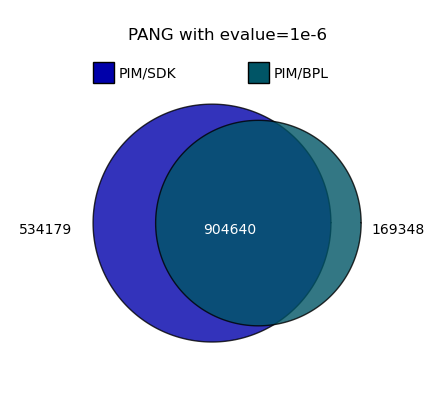
\includegraphics[width=1.1\textwidth]{fig_misc/pang.resulte6.png} % second figure itself
    \end{minipage}
    \begin{minipage}{0.32\textwidth}
        \centering
        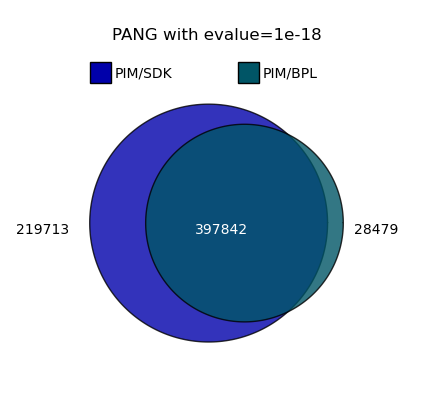
\includegraphics[width=1.1\textwidth]{fig_misc/pang.resulte18.png} % second figure itself
    \end{minipage}
	\caption{Comparing PANG results}
	\label{fig:pang-venn}
\end{figure}

In conclusion, we present several remarks regarding the scalability of the BPL version on multicore and UPMEM architectures. Figure [\ref{fig:pang-scalability}] (left) shows scalability as a function of the number of threads (for multicore) and the number of ranks (for UPMEM). The UPMEM version exhibits good scalability, remaining close to linear, whereas the multicore version shows a noticeable degradation as the number of threads increases. On the right, we analyze the speedup between the multicore and UPMEM versions for an equivalent number of threads/ranks. It can be observed that the UPMEM version benefits from increasing resources, showing improved performance.

\begin{figure}
    \centering
    \begin{minipage}{0.5\textwidth}
        \centering
        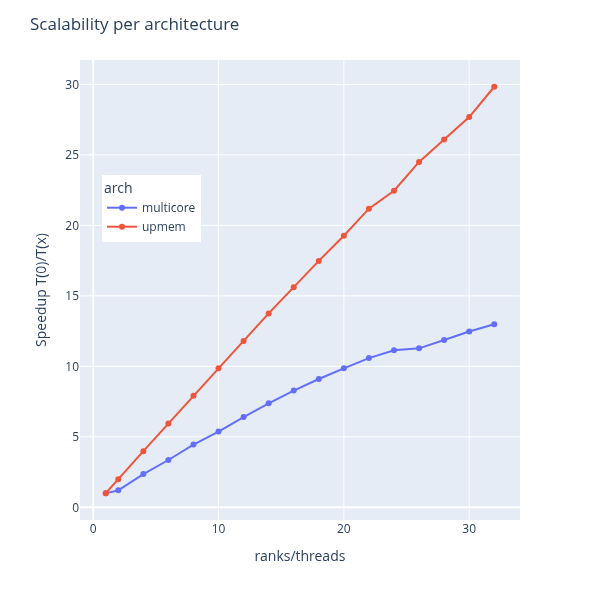
\includegraphics[width=1.0\textwidth]{fig_misc/pang_scalability.png} % first figure itself
    \end{minipage}\hfill
    \begin{minipage}{0.5\textwidth}
        \centering
        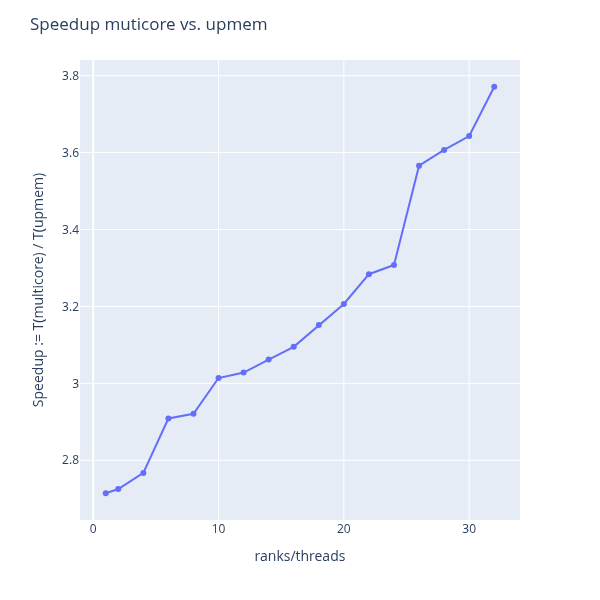
\includegraphics[width=1.0\textwidth]{fig_misc/pang_compare_arch.png} % second figure itself
    \end{minipage}
	\caption{PANG scalability for BPL versions}
	\label{fig:pang-scalability}
\end{figure}

\paragraph{Source code} The BPL implementation is publicly available at \url{https://gitlab.inria.fr/pim/org.pim.pang}.
The UPMEM SDK implementation is publicly available at \url{https://gitlab.inria.fr/pim/pang-sdk}.
